\documentclass[]{article}
\usepackage{lmodern}
\usepackage{amssymb,amsmath}
\usepackage{ifxetex,ifluatex}
\usepackage{fixltx2e} % provides \textsubscript
\ifnum 0\ifxetex 1\fi\ifluatex 1\fi=0 % if pdftex
  \usepackage[T1]{fontenc}
  \usepackage[utf8]{inputenc}
\else % if luatex or xelatex
  \ifxetex
    \usepackage{mathspec}
  \else
    \usepackage{fontspec}
  \fi
  \defaultfontfeatures{Ligatures=TeX,Scale=MatchLowercase}
\fi
% use upquote if available, for straight quotes in verbatim environments
\IfFileExists{upquote.sty}{\usepackage{upquote}}{}
% use microtype if available
\IfFileExists{microtype.sty}{%
\usepackage{microtype}
\UseMicrotypeSet[protrusion]{basicmath} % disable protrusion for tt fonts
}{}
\usepackage[margin=1in]{geometry}
\usepackage{hyperref}
\hypersetup{unicode=true,
            pdfborder={0 0 0},
            breaklinks=true}
\urlstyle{same}  % don't use monospace font for urls
\usepackage{graphicx,grffile}
\makeatletter
\def\maxwidth{\ifdim\Gin@nat@width>\linewidth\linewidth\else\Gin@nat@width\fi}
\def\maxheight{\ifdim\Gin@nat@height>\textheight\textheight\else\Gin@nat@height\fi}
\makeatother
% Scale images if necessary, so that they will not overflow the page
% margins by default, and it is still possible to overwrite the defaults
% using explicit options in \includegraphics[width, height, ...]{}
\setkeys{Gin}{width=\maxwidth,height=\maxheight,keepaspectratio}
\IfFileExists{parskip.sty}{%
\usepackage{parskip}
}{% else
\setlength{\parindent}{0pt}
\setlength{\parskip}{6pt plus 2pt minus 1pt}
}
\setlength{\emergencystretch}{3em}  % prevent overfull lines
\providecommand{\tightlist}{%
  \setlength{\itemsep}{0pt}\setlength{\parskip}{0pt}}
\setcounter{secnumdepth}{0}
% Redefines (sub)paragraphs to behave more like sections
\ifx\paragraph\undefined\else
\let\oldparagraph\paragraph
\renewcommand{\paragraph}[1]{\oldparagraph{#1}\mbox{}}
\fi
\ifx\subparagraph\undefined\else
\let\oldsubparagraph\subparagraph
\renewcommand{\subparagraph}[1]{\oldsubparagraph{#1}\mbox{}}
\fi

%%% Use protect on footnotes to avoid problems with footnotes in titles
\let\rmarkdownfootnote\footnote%
\def\footnote{\protect\rmarkdownfootnote}

%%% Change title format to be more compact
\usepackage{titling}

% Create subtitle command for use in maketitle
\providecommand{\subtitle}[1]{
  \posttitle{
    \begin{center}\large#1\end{center}
    }
}

\setlength{\droptitle}{-2em}

  \title{}
    \pretitle{\vspace{\droptitle}}
  \posttitle{}
    \author{}
    \preauthor{}\postauthor{}
    \date{}
    \predate{}\postdate{}
  
\usepackage{booktabs}
\usepackage{longtable}
\usepackage{array}
\usepackage{multirow}
\usepackage{wrapfig}
\usepackage{float}
\usepackage{colortbl}
\usepackage{pdflscape}
\usepackage{tabu}
\usepackage{threeparttable}
\usepackage{threeparttablex}
\usepackage[normalem]{ulem}
\usepackage{makecell}
\usepackage{xcolor}

\pagenumbering{gobble}
\usepackage{placeins}
\usepackage{float}
\usepackage{caption}
\captionsetup[figure]{labelformat = empty}
\usepackage{xcolor}
\definecolor{link}{rgb}{0, 0, 238}
\usepackage{booktabs}

\begin{document}

{
\setcounter{tocdepth}{5}
\tableofcontents
}
\hypertarget{critical-element-3---technical-quality-validity}{%
\subsection{Critical Element 3 - Technical Quality:
Validity}\label{critical-element-3---technical-quality-validity}}

\hypertarget{overall-validity-including-validity-based-on-content}{%
\subsubsection{3.1 Overall Validity, Including Validity Based on
Content}\label{overall-validity-including-validity-based-on-content}}

As elaborated by Messick (1989), the validity argument involves a claim
with evidence evaluated to make a judgment. Three essential components
of assessment systems are necessary: (a) constructs (what to measure),
(b) the assessment instruments and processes (approaches to
measurement), and (c) use of the test results (for specific
populations). Validation is a judgment call on the degree to which each
of these components is clearly defined and adequately implemented.

Validity is a unitary concept with multifaceted processes of reasoning
about a desired interpretation of test scores and subsequent uses of
these test scores. In this process, we want answers for two important
questions. Regardless of whether the students tested have disabilities,
the questions are identical: (1) How valid is our interpretation of a
student's test score? and (2) How valid is it to use these scores in an
accountability system? Validity evidence may be documented at both the
item and total test levels. We use the Standards (AERA et al., 2014) in
documenting evidence on content coverage, response processes, internal
structure, and relations to other variables. This document follows the
essential data requirements of the federal government as needed in the
peer review process. The critical elements highlighted in Section 4 in
that document (with examples of acceptable evidence) include (a)
academic content standards, (b) academic achievement standards, (c) a
statewide assessment system, (d) reliability, (e) validity, and (f)
other dimensions of technical quality.

In this technical report, data are presented to support the claim that
Oregon's AA-AAAS provides the state technically adequate student
performance data to ascertain proficiency on grade level state content
standards for students with significant cognitive disabilities - which
is its defined purpose. The AA-AAAS are linked to grade level academic
content, generate reliable outcomes at the test level, include all
students, have a cogent internal structure, and fit within a network of
relations within and across various dimensions of content related to and
relevant for making proficiency decisions. Sample items that convey the
design and sample content of ORExt items are provided in \emph{Appendix}
2.2.3.

The assessments are administered and scored in a standardized manner.
Assessors who administer the ORExt are trained to provide the necessary
level of support for appropriate test administration on an item-by-item
basis. There are four levels of support outlined in training: full
physical support, partial physical support, prompted support, and no
support. Items were designed to document students' skill and knowledge
on grade level academic content standards, with the level of support
provided designed not to interfere with the construct being measured.
Only one test administration type is used for the ORExt, patterned after
the former Scaffold version of the assessment. Assessors administer the
prompt and if the student does not respond, the Assessor reads a
directive statement designed to focus the student's attention upon the
test item and then repeats the prompt. If the student still does not
respond, the Assessor repeats the prompt as needed and otherwise scores
the item as incorrect and moves on to the next item. Training
documentation is provided in \emph{Appendices} 2.3B.1-2.3B.8.

Given the content-related evidence that we present related to test
development, alignment, training, administration, scoring, the
reliability information reflected by adequate coefficients for tests,
and, finally, the relation of tests across subject areas (providing
criterion-related evidence), we conclude that the alternate assessment
judged against alternate achievement standards allows valid inferences
to be made on state accountability proficiency standards.

\hypertarget{a-alignment-between-aa-aaas-and-academic-content-standards}{%
\paragraph{3.1A Alignment Between AA-AAAS and Academic Content
Standards}\label{a-alignment-between-aa-aaas-and-academic-content-standards}}

Our foundation of validity evidence from content coverage for the ORExt
comes in the form of test specifications (see \emph{Appendix} 2.1) and
test blueprints (see \emph{Appendix} 2.1B). Among other things, the
Standards (AERA et al., 2014) suggest specifications should ``define the
content of the test, the proposed test length, the item
formats\ldots{}'' (Standard 4.2, p.~85).

All items are linked to grade level standards and a prototype was
developed using principles of universal design with traditional,
content-referenced multiple-choice item writing techniques. The most
important component in these initial steps addressed language complexity
and access to students using both receptive, as well as expressive,
communication. Additionally, both content breadth and depth were
addressed. We developed one test form for the ORExt that utilizes a
scaffold approach. This approach allows for students with very limited
attention to access test content, while the supports are not utilized
for students who do not need this support.

We developed the test iteratively by developing items (see
\emph{Appendix} 2.2.1, which conveys our item writer training
materials), piloting them, reviewing them, and editing successive
drafts. We used a combination of existing panels of veteran teachers who
have worked with the Oregon Department of Education (ODE) in various
advising roles on testing content in general and special education,
using the same processes and criteria, as well as the introduction of
newer teachers who are qualified as we proceed to remain relevant.
Behavioral Research and Teaching (BRT) personnel conducted the internal
reviews of content. After the internal development of prototype items,
all reviews then involved Oregon content and special education experts
with significant training and K-12 classroom experience.

The ORExt incorporates continuous improvement into its test design via
field-testing in all content areas on an annual basis, with an average
of 25\% new items. These items are compared to operational items based
on item functioning and test design factors, generating data used to
replace items on an annual basis, incorporating the new items that fill
a needed gap with regard to categorical concurrence, or provide for a
wider range of functioning with regard to complexity levels: low -
medium - high, comparable to Webb's DOK (see Section 2.2).

BRT employed a multi-stage development process in 2014-15 to ensure that
test items were linked to relevant content standards, were accessible
for students with significant cognitive disabilities, and that any
perceived item biases were eliminated. The item review process included
51 reviewers with an average of 22 years of experience in education. The
ORExt assessments have been determined to demonstrate strong linkage to
grade level academic content, overall. Full documentation of the initial
2014 linkage study and a new, independent alignment study conducted in
spring, 2017 is provided in \emph{Appendix} 3.1A. Based on student
performance from the 2016-2017 testing year, new and Grade 7 Math field
test items were written in fall 2017.

The summary section of the independent alignment study report states
that, ``Oregon's Extended Assessments (ORExt) in English Language Arts,
Mathematics, and Science were evaluated in a low-complexity alignment
study conducted in Spring of 2017. Averages of reviewer professional
judgments over five separate evaluations were gathered, reviewed, and
interpreted in the pages that follow. In the three evaluations that
involved determining the relationship between standards and items,
reviewers identified sufficient to strong relationships among assessment
components in all grades and all subject areas. In the two evaluations
involving Achievement Level Descriptors, reviewers identified thirty
instances of sufficient to strong relationships out of thirty-four
possible relationship opportunities resulting in an overall affirmed
relationship with areas for refinements identified.''

Because the assessments demonstrate sufficient to strong linkage to
Oregon's general education content standards and descriptive statistics
demonstrate that each content area assessment is functioning as
intended, it is appropriate to deduce that these standards define the
expectations that are being measured by the Oregon Extended assessments.

The Oregon Extended assessments yield scores that reflect the full range
of achievement implied by Oregon's alternate achievement standards.
Evidence of this claim is found in the standard setting documentation
submitted in Section 6.2. Standards were set for all subject areas on
June 15-17, 2015. Standards included achievement level descriptors and
cut scores, which define Oregon's new alternate achievement standards
(AAS). The State Board of Education officially adopted the AAS on June
25, 2015.

\hypertarget{b-aa-aaas-linkage-to-general-content-standards}{%
\paragraph{3.1B AA-AAAS Linkage to General Content
Standards}\label{b-aa-aaas-linkage-to-general-content-standards}}

Results of the analysis of the linkage of the new Essentialized
Assessment Frameworks, (EAF), composed of Essentialized Standards
(EsSt), to grade level CCSS in English language arts and mathematics and
linked to ORSci and NGSS in science, are presented in Section 3.1A. The
claim is that the EsSt are sufficiently linked to grade level standards,
while the ORExt items are aligned to the EsSt. In addition to presenting
linkage information between grade level content standards and the EsSt,
the linkage study presents alignment information related to the items on
the new ORExt in comparison to the EsSt. Extended assessments have been
determined to link sufficiently to grade level academic content
standards. Field test items are added each year based on item alignment
to standards.

The Oregon Extended assessments link to grade level academic content, as
reflected in the item development process. Oregon also had each
operational item used on the Oregon Extended assessment evaluated for
alignment as part of two comprehensive linkage studies, one performed in
2014 and an independent alignment study performed in 2017 (see Section
3.1A). The professional reviewers in an internal study in 2014 and an
independent study in spring 2017 included both special and general
education experts, with content knowledge and experience in addition to
special education expertise.

According to the independent linkage study report, the spring 2017
review was conducted by expert reviewers with professional backgrounds
in either Special Education (the population), Assessment, or in Oregon's
adopted content standards. Reviewers were assigned to review grade-level
items relative to their experience and expertise. In all, 39 reviewers
participated. Thirty-four (34) participated in all 5 evaluations:
thirteen (13), for the English Language Arts review, fifteen (15) for
the Mathematics review, and six (6) for the Science review. All
participants were assigned to at least one specific content area as
shown in Table 1. Note: Four individuals were assigned to two areas of
review. The thirty-nine individuals who participated in the study had a
robust legacy of experience in the field and in the state. Participants
represented 25 unique school districts across the state representing
both urban and rural perspectives. All 39 of the individuals
participating in the study held current teaching licenses. Two
individuals also held administrative licenses. Years of experience in
their area ranged from 3 - 30 years of experience with an average of 17
years of experience. (Mode = 11 years, Median = 16 years). One
individual indicated 50 years of experience in the field. Three of the
39 individuals held a Bachelor's degree only. Thirty-six held a
Bachelor's degree and at least one Master's degree. Two held a
Bachelor's degree, at least one Master's degree, and a doctoral degree.
Fourteen (36\%) of the individuals identified as experts in a specific
Content area and 25 (64\%) of the individuals identified Special
education as their primary area of expertise.

These skilled reviewers were trained by synchronous webinars on
linkage/alignment, as well as item depth, breadth, and complexity and
then completed their ratings online via BRT's Distributed Item Review
(DIR) website and on Excel spreadsheets shared with the researcher
electronically (see \emph{Appendix} 3.1B for an overview). Mock linkage
ratings were conducted in order to address questions and ensure
appropriate calibration. Reviewers rated each essentialized standard on
a 3-point scale (0 = no link, 1= sufficient link, 2= strong link) as it
related to the standard the test developers had defined for that
essentialized standard. Items were evaluated, in turn, based upon their
alignment to the essentialized standard on a 3-point scale (0 =
insufficient alignment, 1 = sufficient alignment, 2 = strong alignment).
When averaged across reviewers, 1.00-1.29 was considered in the low
range, 1.30 - 1.69 was sufficient, and 1.70 - 2.0 was strong. Additional
comment was requested for any essentialized standard or item whose
linkage was rated 0.

Overall, the 2017 independent alignment study concludes that: ``First,
reviewers were asked to conduct an affirmational review of the rationale
used by test developers to omit certain content standards. This finding
was used to infer that the final standards selected for inclusion or
omission in Oregon's Extended Assessment were chosen rationally and that
the final scope of content standards can be considered justifiable for
the population for the subject area. Conclusion: This review, with a
lowest average rate of .82 (on a scale of 1), permits the inference: the
scope of the standards selected for translation to Essentialized
Standards were rationally selected. None of the standards de-selected
(for inaccessibility or for being covered elsewhere) were strongly
identified for re- inclusion, nor were identified as a critical hole for
this population of students. Second, reviewers were asked to identify
the strength of the link between the source standard and the
Essentialized Standard. This finding was used to infer that the process
undertaken to essentialize a given Source Standard did not fundamentally
or critically alter the knowledge or skill set intended by the source
standard for this population of students (further confirming that the
content selected for assessment is comparable). Conclusion:This review,
with a range of 1.5 - 1.9 (on a scale of 2) permits the inference: the
Essentialized Standards were found to link sufficiently to the source
standards on average beyond the''sufficient" average of 1.0. Third,
reviewers were asked to identify the strength of the alignment between
the Essentialized Standards and the items and to review the items
developed using the Essentialized Standards for bias, and accessibility.
The finding from this review was used to infer that the items written
for this grade and subject area (using these Essentialized Standards)
were adequately linked to the Essentialized Standards, were free from
bias, and were accessible to students with significant cognitive
disabilities. Conclusion: The alignment review (1.32 - 1.89),
accessibility review (.67 - 1.0), and freedom from bias review (.65 -
1.0) all permit the inference that the test items indicate a
relationship with the source standards, the test items are not overly
biased towards or against any particular group of individuals, and the
test items are written such that the content and intent can be accessed
by students with the most significant cognitive disabilities. (**Note:
this range was skewed by feedback from one reviewer --ELA-Grade 3 -
whose comments were noted in this study. Removing that individual's
comments would result in a range of .90 - 1.0 accessibility range and
.89 - 1.0 freedom from bias range respectively.) Fourth, reviewers were
asked to review the statements used to describe student achievement on
the test (the Achievement Level Descriptors) and their alignment to the
Essentialized Standards that the students were tested on. The finding
from this review was used to infer that the skills and achievements
described by the Achievement Level Descriptors for each subject and
grade level are aligned with the content standard being measured.
Conclusion: The reviews ranging from .68* - 1.0 permit the inference
that the descriptions made regarding student skillset are an accurate
reflection of the standards from which the assessment was developed at
all three levels evaluated. (*One outlier for ELA-Grade 4 provided a
review of a .52 average). Fifth, and finally, reviewers were asked to
review the alignment of the Achievement Level Descriptors to the items.
The finding from this review was used to infer that each item in the
developed assessment(s) was appropriately aligned to its associated
Achievement Level Descriptor (further confirming that decisions made
using this test were aligned with the intent of the source standard).
Conclusion: Fourteen of the seventeen grade-level reviews resulted in an
average reviewer range of .67 - 1.0 indicating an appropriate alignment
between ALDs and the items as written. This review permits the inference
that, overall, the Achievement Level Descriptors are accurate
reflections of the items. In three instances (Mathematics-Grades 3 and
4, and ELA-Grade 8) the average alignment by reviewer was .5 (indicating
that one of the two individuals in that category did not agree that the
items and ALDs were aligned)."

\hypertarget{validity-based-on-cognitive-processes}{%
\subsubsection{3.2 Validity Based on Cognitive
Processes}\label{validity-based-on-cognitive-processes}}

Evidence of content coverage is concerned with judgments about ``the
extent to which the content domain of a test represents the domain
defined in the test specifications'' (AERA et al., 2014, Standard 4.12,
p.~89). As a whole, the ORExt is comprised of sets of items that sample
student performance on the intended domains. The expectation is that the
items cover the full range of intended domains, with a sufficient number
of items so that scores credibly represent student knowledge and skills
in those areas. Without a sufficient number of items, the potential
exists for a validity threat due to construct under-representation
(Messick, 1989).

The ORExt assessment is built upon a variety of items that address a
wide range of performance expectations rooted in the CCSS, NGSS, and
ORSci content standards. The challenge built into the test design is
based first upon the content within each standard in English language
arts, mathematics, and science. That content is RDBC in a manner that is
verified by Oregon general and special education teachers to develop
assessment targets that are appropriate for students with the most
significant cognitive disabilities. Our assessments utilize universal
design principles in order to include all students in the assessment
process, while effectively challenging the higher performing students.
For students who have very limited to no communication and are unable to
access even the most accessible items on the ORExt, an Oregon
Observational Rating Assessment (ORora) was first implemented in
2015-16. The ORora is completed by teachers and documents the student's
level of communication complexity (expressive and receptive), as well as
level of independence in the domains of attention/joint attention and
mathematics. A complete report of ORora results from 2017-18 is provided
in \emph{Appendix} 5.1D.

Fifty-one reviewers analyzed all ORExt items for bias, sensitivity,
accessibility to the student population, and alignment to the
Essentialized Standards. A total of 21 reviewers were involved in the
English language arts item reviews. An additional 21 reviewers were
involved in the Mathematics item reviews. Science employed nine
reviewers. Reviewers were organized into grade level teams of two
special educators and one content specialist.

Substantive evidence that has been documented suggests that the ORExt
items are tapping the intended cognitive processes and that the items
are at the appropriate grade level through the linkage/alignment studies
documented above, including reviews of linkage, content coverage, and
depth of knowledge.

\hypertarget{validity-based-on-internal-structure-content-and-function}{%
\subsubsection{3.3 Validity Based on Internal Structure (Content and
Function)}\label{validity-based-on-internal-structure-content-and-function}}

The Oregon Extended assessments reflect patterns of emphasis that are
supported by Oregon educators as indicated by the following three tables
that highlight the balance of standard representation by grade level for
English language arts, mathematics, and science on the ORExt. The
representation ratios can be calculated by dividing the standards by the
total within each respective column. For example, in Grade 3 Reading,
approximately 25\% of the items are in the Reading Standards for
Literature domain, as that domain has 4 written Essentialized Standards
(EsSt) out of the total of 16 (4/16 = 25\%).

The test blue prints below directly correspond to the number of ES
written in each domain within the Essentialized Assessment Frameworks
(EAF) spreadsheets. There are additional grade level standards addressed
by the EsSt, as some EsSt link to multiple grade level content
standards. However, the blueprints below reflect only the written EsSt
and are thus an underrepresentation of the breadth of grade level
content addressed by the ORExt.\FloatBarrier
\includegraphics{Figures/EsSt/EsStELA.png} \FloatBarrier
\includegraphics{Figures/EsSt/EsStMathScience.png} The primary purpose
of the ORExt assessment is to yield technically adequate performance
data on grade level state content standards for students with
significant cognitive disabilities in English language arts,
mathematics, and science at the test level. All scoring and reporting
structures mirror this design and have been shown to be reliable
measures at the test level (see Section 4.1). The process of addressing
any gaps or weaknesses in the system is accomplished via field-testing
(see Section 3.1A).

\hypertarget{point-measure-correlations}{%
\paragraph{Point Measure
Correlations}\label{point-measure-correlations}}

Distributions of point measure correlations and outfit mean square
statistics for operational items are provided below, by content area and
grade. Point measure correlations display how the item scores correlate
with the latent overall score, while outfit mean square statistics
closer to 1.0 denote minimal distortion of the measurement system. All
items included in the 2017-18 operational assessment are represented.
Point measure correlations ranged from 0.34 to 0.74 in ELA, 0.12 to 0.71
in Math, to 0.25 to 0.74 in Science. All data visualizations were
conducted with \emph{ggplot} in the \emph{tidyverse} package (Wickham,
H., 2017).

\begin{table}[!h]

\caption{\label{tab:ifiles}Point Measure Correlations: English/Language Arts}
\centering
\begin{tabu} to \linewidth {>{\raggedleft}X>{\raggedleft}X>{\raggedleft}X>{\raggedleft}X}
\toprule
Grade & Mean & Min & Max\\
\midrule
3 & 0.57 & 0.37 & 0.70\\
4 & 0.59 & 0.24 & 0.73\\
5 & 0.63 & 0.46 & 0.71\\
6 & 0.62 & 0.47 & 0.72\\
7 & 0.60 & 0.35 & 0.69\\
\addlinespace
8 & 0.61 & 0.41 & 0.74\\
11 & 0.68 & 0.57 & 0.76\\
\bottomrule
\end{tabu}
\end{table}
\begin{table}[!h]

\caption{\label{tab:ifiles}Point Measure Correlations: Math}
\centering
\begin{tabu} to \linewidth {>{\raggedleft}X>{\raggedleft}X>{\raggedleft}X>{\raggedleft}X}
\toprule
Grade & Mean & Min & Max\\
\midrule
3 & 0.49 & 0.06 & 0.68\\
4 & 0.46 & 0.20 & 0.71\\
5 & 0.45 & 0.23 & 0.65\\
6 & 0.52 & 0.28 & 0.73\\
7 & 0.46 & 0.04 & 0.71\\
\addlinespace
8 & 0.42 & 0.12 & 0.66\\
11 & 0.54 & 0.42 & 0.71\\
\bottomrule
\end{tabu}
\end{table}
\begin{table}[!h]

\caption{\label{tab:ifiles}Point Measure Correlations: Science}
\centering
\begin{tabu} to \linewidth {>{\raggedleft}X>{\raggedleft}X>{\raggedleft}X>{\raggedleft}X}
\toprule
Grade & Mean & Min & Max\\
\midrule
5 & 0.61 & 0.20 & 0.73\\
8 & 0.64 & 0.38 & 0.72\\
11 & 0.68 & 0.31 & 0.76\\
\bottomrule
\end{tabu}
\end{table}

\hypertarget{outfit-mean-square-distributions}{%
\paragraph{Outfit Mean Square
Distributions}\label{outfit-mean-square-distributions}}

Outfit mean square values below 1.0 demonstrate that values are too
predictable and perhaps redundant, while values above 1.0 indicate
unpredictability. Items above 2.0 are deemed insufficient for
measurement purposes and flagged for replacement. While most OMS values
in ELA were between 0.5 and 1.5, one item in each Grade 6, 7, and 11 was
above 2.0 and will be removed. One item in Grade 7 Math and one item in
Grade 11 Science will also be removed.

\begin{table}[!h]

\caption{\label{tab:outfit}Mean Square Outfit: English/Language Arts}
\centering
\begin{tabu} to \linewidth {>{\raggedleft}X>{\raggedleft}X>{\raggedleft}X>{\raggedleft}X}
\toprule
Grade & Mean & Min & Max\\
\midrule
3 & 0.96 & 0.56 & 1.67\\
4 & 0.99 & 0.60 & 4.92\\
5 & 1.03 & 0.61 & 3.31\\
6 & 0.97 & 0.53 & 1.93\\
7 & 1.00 & 0.63 & 2.20\\
\addlinespace
8 & 0.95 & 0.49 & 1.72\\
11 & 0.96 & 0.43 & 2.86\\
\bottomrule
\end{tabu}
\end{table}
\begin{table}[!h]

\caption{\label{tab:outfit}Mean Square Outfit: Math}
\centering
\begin{tabu} to \linewidth {>{\raggedleft}X>{\raggedleft}X>{\raggedleft}X>{\raggedleft}X}
\toprule
Grade & Mean & Min & Max\\
\midrule
3 & 0.98 & 0.68 & 2.33\\
4 & 0.97 & 0.70 & 1.33\\
5 & 1.09 & 0.63 & 2.86\\
6 & 0.91 & 0.49 & 1.58\\
7 & 1.05 & 0.55 & 3.22\\
\addlinespace
8 & 1.00 & 0.64 & 1.71\\
11 & 0.99 & 0.62 & 1.40\\
\bottomrule
\end{tabu}
\end{table}
\begin{table}[!h]

\caption{\label{tab:outfit}Mean Square Outfit: Science}
\centering
\begin{tabu} to \linewidth {>{\raggedleft}X>{\raggedleft}X>{\raggedleft}X>{\raggedleft}X}
\toprule
Grade & Mean & Min & Max\\
\midrule
5 & 1.00 & 0.49 & 2.73\\
8 & 0.90 & 0.56 & 1.58\\
11 & 0.88 & 0.45 & 2.28\\
\bottomrule
\end{tabu}
\end{table}

\hypertarget{annual-measureable-objectives-frequencies-percentages}{%
\paragraph{Annual Measureable Objectives Frequencies \&
Percentages}\label{annual-measureable-objectives-frequencies-percentages}}

Annual Measurable Objective (AMO) calculations were conducted based upon
student performance on the ORExt tied to the vertical scale using Rasch
modeling. Overall results are largely consistent with 2016-17, with
approximately 50\% of students with significant cognitive disabilities
achieving proficiency across grades and content areas. The data
visualizations presented below were conducted with ggplot in the
tidyverse package (Wickham, H., 2017).

\begin{table}[!h]

\caption{\label{tab:ode_data}English/Language Arts Percent Proficient By Grade}
\centering
\begin{tabu} to \linewidth {>{\raggedright}X>{\raggedleft}X>{\raggedleft}X>{\raggedleft}X>{\raggedleft}X}
\toprule
Grade & AMO Level 1 & AMO Level 2 & AMO Level 3 & AMO Level 4\\
\midrule
Grade 3 & 20 & 42 & 28 & 10\\
Grade 4 & 29 & 27 & 26 & 18\\
Grade 5 & 27 & 32 & 18 & 23\\
Grade 6 & 30 & 28 & 23 & 19\\
Grade 7 & 31 & 29 & 25 & 16\\
\addlinespace
Grade 8 & 41 & 24 & 24 & 11\\
Grade 11 & 23 & 28 & 11 & 39\\
Grade 12 & 12 & 19 & 12 & 57\\
\bottomrule
\end{tabu}
\end{table}
\begin{table}[!h]

\caption{\label{tab:ode_data}Math Percent Proficient By Grade}
\centering
\begin{tabu} to \linewidth {>{\raggedright}X>{\raggedleft}X>{\raggedleft}X>{\raggedleft}X>{\raggedleft}X}
\toprule
Grade & AMO Level 1 & AMO Level 2 & AMO Level 3 & AMO Level 4\\
\midrule
Grade 3 & 42 & 18 & 35 & 5\\
Grade 4 & 31 & 40 & 23 & 6\\
Grade 5 & 25 & 34 & 34 & 7\\
Grade 6 & 51 & 10 & 32 & 8\\
Grade 7 & 57 & 7 & 31 & 5\\
\addlinespace
Grade 8 & 49 & 16 & 34 & 1\\
Grade 11 & 42 & 16 & 32 & 10\\
Grade 12 & 29 & 20 & 29 & 22\\
\bottomrule
\end{tabu}
\end{table}
\begin{table}[!h]

\caption{\label{tab:ode_data}Reading Percent Proficient By Grade}
\centering
\begin{tabu} to \linewidth {>{\raggedright}X>{\raggedleft}X>{\raggedleft}X>{\raggedleft}X>{\raggedleft}X}
\toprule
Grade & AMO Level 1 & AMO Level 2 & AMO Level 3 & AMO Level 4\\
\midrule
Grade 3 & 20 & 40 & 30 & 9\\
Grade 4 & 24 & 30 & 28 & 18\\
Grade 5 & 28 & 34 & 16 & 21\\
Grade 6 & 32 & 22 & 26 & 20\\
Grade 7 & 30 & 29 & 18 & 23\\
\addlinespace
Grade 8 & 41 & 25 & 25 & 9\\
Grade 11 & 24 & 23 & 13 & 41\\
Grade 12 & 12 & 21 & 12 & 55\\
\bottomrule
\end{tabu}
\end{table}
\begin{table}[!h]

\caption{\label{tab:ode_data}Science Percent Proficient By Grade}
\centering
\begin{tabu} to \linewidth {>{\raggedright}X>{\raggedleft}X>{\raggedleft}X>{\raggedleft}X>{\raggedleft}X}
\toprule
Grade & AMO Level 1 & AMO Level 2 & AMO Level 3 & AMO Level 4\\
\midrule
Grade 5 & 37 & 20 & 23 & 21\\
Grade 8 & 42 & 16 & 22 & 20\\
Grade 11 & 23 & 17 & 26 & 34\\
Grade 12 & 16 & 11 & 26 & 47\\
\bottomrule
\end{tabu}
\end{table}
\begin{table}[!h]

\caption{\label{tab:ode_data}Writing Percent Proficient By Grade}
\centering
\begin{tabu} to \linewidth {>{\raggedright}X>{\raggedleft}X>{\raggedleft}X>{\raggedleft}X>{\raggedleft}X}
\toprule
Grade & AMO Level 1 & AMO Level 2 & AMO Level 3 & AMO Level 4\\
\midrule
Grade 3 & 26 & 31 & 26 & 17\\
Grade 4 & 33 & 20 & 34 & 14\\
Grade 5 & 36 & 28 & 9 & 28\\
Grade 6 & 29 & 27 & 24 & 19\\
Grade 7 & 37 & 29 & 18 & 15\\
\addlinespace
Grade 8 & 46 & 14 & 19 & 21\\
Grade 11 & 23 & 28 & 7 & 41\\
Grade 12 & 14 & 21 & 5 & 60\\
\bottomrule
\end{tabu}
\end{table}

\clearpage

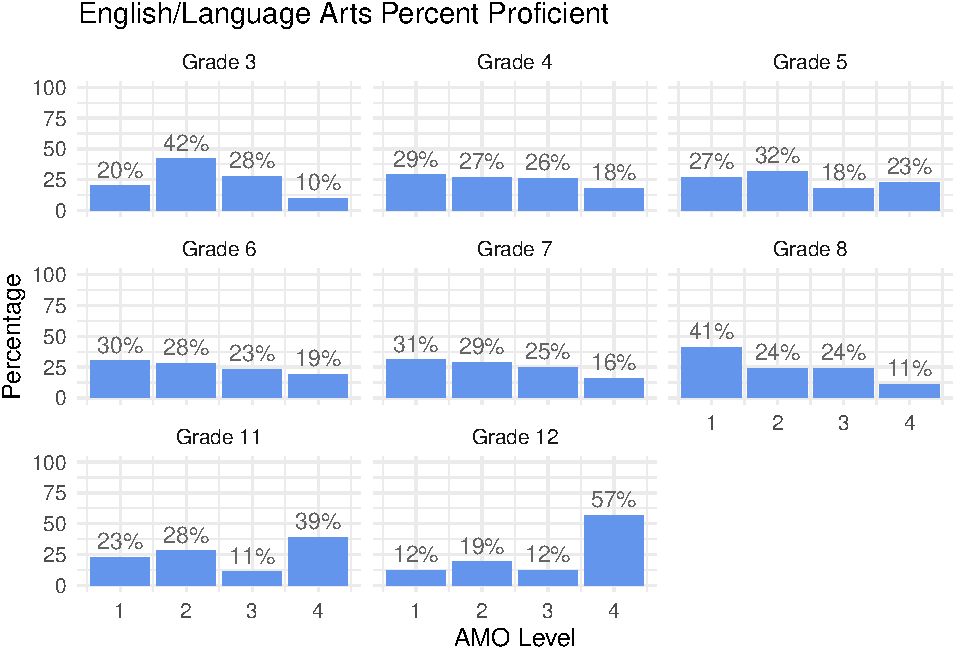
\includegraphics{Critical_Element_3_files/figure-latex/amo_plot-1.pdf}
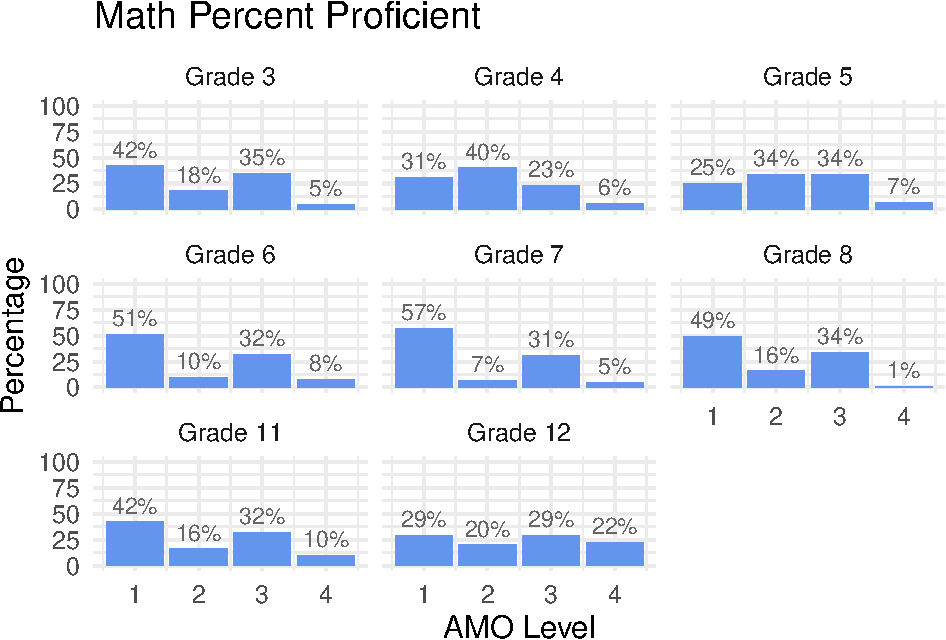
\includegraphics{Critical_Element_3_files/figure-latex/amo_plot-2.pdf}
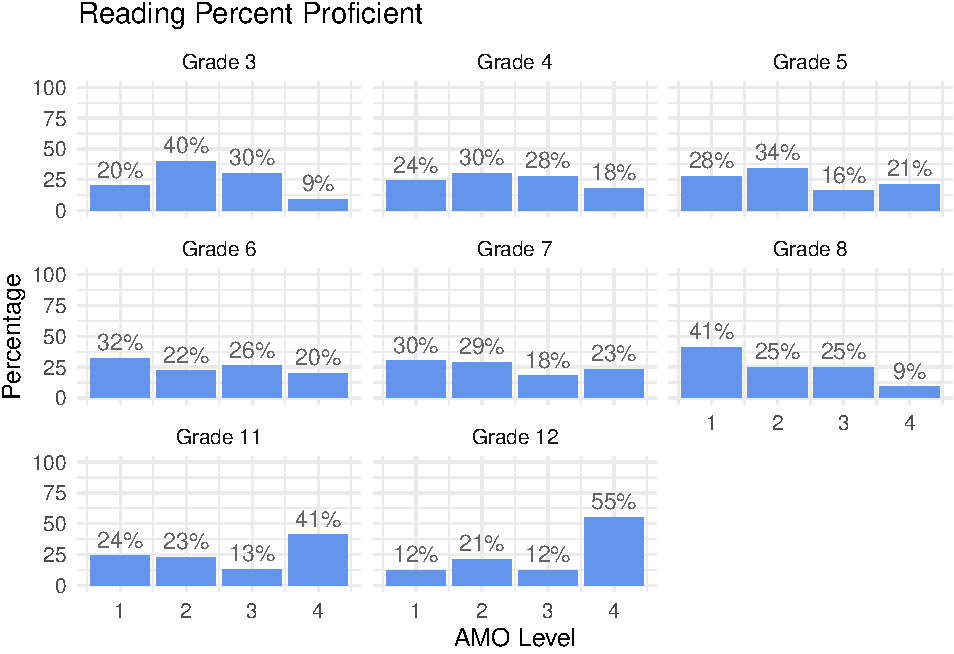
\includegraphics{Critical_Element_3_files/figure-latex/amo_plot-3.pdf}
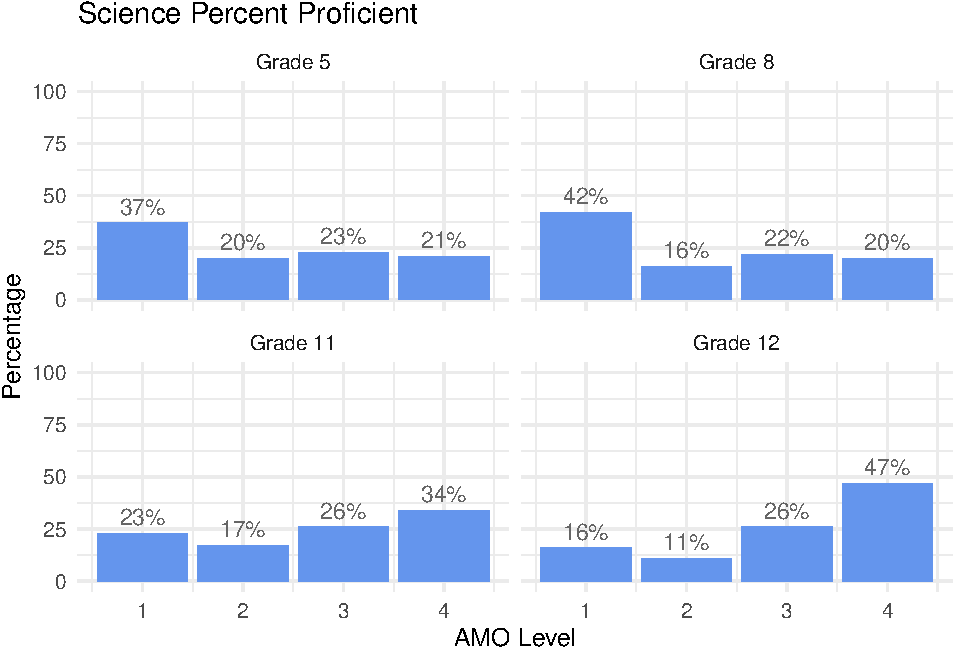
\includegraphics{Critical_Element_3_files/figure-latex/amo_plot-4.pdf}
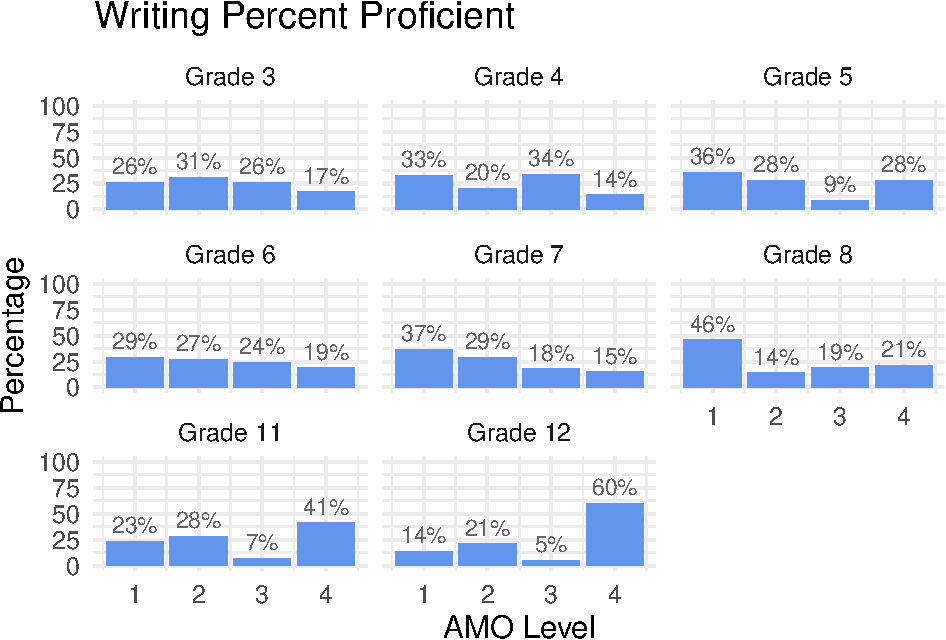
\includegraphics{Critical_Element_3_files/figure-latex/amo_plot-5.pdf}

Some concerns are noted in mathematics, where relatively higher
percentages of students are scoring at Level 1 and very few at Level 2.
However, this finding is consistent with the range of possible scores,
where Level 2 in some cases only has two possible scale score points
(e.g., Grade 7, where Level 2 exists between 207-208 scaled scores). The
addition of 1-2 low complexity items per assessment will be effected in
mathematics to address this concern, as well.

\hypertarget{validity-based-on-relations-to-other-variables}{%
\subsubsection{3.4 Validity Based on Relations to Other
Variables}\label{validity-based-on-relations-to-other-variables}}

Perhaps the best model for understanding criterion-related evidence
comes from Campbell and Fiske (1959) in their description of the
multi-trait, multi-method analysis {[}we translate the term `trait' to
mean `skill'{]}. In this process (several) different traits are measured
using (several) different methods to provide a correlation matrix that
should reflect specific patterns supportive of the claim being made
(that is, provide positive validation evidence). Sometimes, these
various measures are of the same or similar skills, abilities, or
traits, and other times they are of different skills, abilities, or
traits. We present data that quite consistently reflect higher relations
among items within an academic subject than between academic subjects.
We also present data in which performance on items is totaled within
categories of disability, expecting relations that would reflect
appropriate differences (see Tindal, McDonald, Tedesco, Glasgow, Almond,
Crawford, \& Hollenbeck, 2003).

\hypertarget{convergent-and-divergent-validity-documentation}{%
\paragraph{Convergent and Divergent Validity
Documentation}\label{convergent-and-divergent-validity-documentation}}

Criterion validity information is difficult to document with AA-AAAS, as
most SWSCD do not participate in any standardized assessment outside of
the ORExt and/or ORora in Oregon. Divergent validity evidence is
garnered via comparisons of ORExt results to ORora outcomes shows that
students whose ORExt assessments are discontinued exhibit serious
limitations in attention, basic math skills, and receptive and
expressive communication skills. The median ORExt ELA score for SWSCD
who participated in the ORora was 4.0. The median mathematics ORExt
score was 4.0, and the median science ORExt score for SWSCD who were
evaluated with the ORora was 0.0. Pearson correlations between the total
raw scores on the ORExt and the total raw score on the ORora were
conducted to address the relationship between total performance on each
assessment. The correlation between ELA and ORora scores was 0.56,
between Math and ORora scores was 0.52, and between Science and ORora
scores was 0.33. As expected, the ORora results provide divergent
validity evidence for the ORExt. We would not expect a strong
relationship between the scores, as students whose ORExt testing is
discontinued are generally unable to access the academic content on the
ORExt, even with the requisite reductions in depth, breadth, and
complexity.

Convergent evidence that the ORExt is assessing appropriate academic
content is provided by QA and QT responses to the consequential validity
survey. Respondents to the survey generally agree that, ``The items in
the Oregon Extended Assessment accurately reflect the academic content
(what the student should know) that my students with significant
cognitive disabilities should be learning, as defined by grade level
content standards (CCSS/NGSS) and the Essentialized Assessment
Frameworks'' (85\% Strongly Agree or Agree). In addition, they also
agreed with the statement that, ``The items in the Oregon Extended
Assessment, which primarily ask students to match, identify, or
recognize academic content, are appropriate behaviors to review to
determine what my students with significant cognitive disabilities are
able to do'' (85\% Strongly Agree or Agree). The consequential validity
results demonstrate that the ORExt is sampling academic domains that the
field of QAs and QTs deem appropriate in the area of academics. See
\emph{Appendix} 2.3B.10 for complete consequential vailidity study
results.

\hypertarget{analyses-within-and-across-subject-areas}{%
\paragraph{Analyses Within and Across Subject
Areas}\label{analyses-within-and-across-subject-areas}}

We conducted correlational analyses to further explore the validity of
the ORExt. We first describe the purpose of the analysis, as well as our
anticipated results. We then discuss our observed results before
concluding with an overall evaluative judgment of the validity of the
test.

In the correlational analysis, we explore the correlations among
students' total scores across subject areas. The purpose of the analysis
was to investigate how strongly students' scores in one area were
related to students' scores in other subject areas. If the correlations
were exceedingly high (e.g., above .90), it would indicate that the
score a student receives in an individual subject has less to do with
the intended construct (i.e., reading) than with factors idiosyncratic
to the student. For example, if all subject areas correlated at .95,
then it would provide strong evidence that the tests would be measuring
a global student-specific construct (i.e., intelligence), and not the
individual subject constructs. We would expect, however, that the tests
would correlate quite strongly given that the same students were
assessed multiple times. Therefore, we would expect moderately strong
correlations (e.g., 0.7) simply because of the within-subject design.
Idiosyncratic variance associated with the individual student is thus
captured.

\hypertarget{correlational-analyses-results}{%
\paragraph{Correlational Analyses
Results}\label{correlational-analyses-results}}

Full results of the Pearson's product-moment correlation analysis by
content area and grade level are reported below. The results are
significant, yet the overall correlations across content areas suggest
that we are indeed measuring different, though strongly related
constructs, with between-test scaled score correlations ranging from
0.69 to 0.97.

\newpage
\begin{table}[!h]

\caption{\label{tab:by_sub_corr}Grade 3 Content Area Correlations}
\centering
\begin{tabu} to \linewidth {>{\raggedright}X>{\raggedleft}X>{\raggedleft}X>{\raggedleft}X>{\raggedleft}X}
\toprule
Variable & ELA & Math & Reading & Writing\\
\midrule
ELA &  &  &  & \\
Math & 0.84 &  &  & \\
Reading & 0.98 & 0.82 &  & \\
Writing & 0.93 & 0.80 & 0.87 & \\
\bottomrule
\end{tabu}
\end{table}
\begin{table}[!h]

\caption{\label{tab:by_sub_corr}Grade 4 Content Area Correlations}
\centering
\begin{tabu} to \linewidth {>{\raggedright}X>{\raggedleft}X>{\raggedleft}X>{\raggedleft}X>{\raggedleft}X}
\toprule
Variable & ELA & Math & Reading & Writing\\
\midrule
ELA &  &  &  & \\
Math & 0.83 &  &  & \\
Reading & 0.97 & 0.81 &  & \\
Writing & 0.93 & 0.74 & 0.84 & \\
\bottomrule
\end{tabu}
\end{table}
\begin{table}[!h]

\caption{\label{tab:by_sub_corr}Grade 5 Content Area Correlations}
\centering
\begin{tabu} to \linewidth {>{\raggedright}X>{\raggedleft}X>{\raggedleft}X>{\raggedleft}X>{\raggedleft}X>{\raggedleft}X}
\toprule
Variable & ELA & Math & Reading & Science & Writing\\
\midrule
ELA &  &  &  &  & \\
Math & 0.81 &  &  &  & \\
Reading & 0.98 & 0.78 &  &  & \\
Science & 0.81 & 0.77 & 0.79 &  & \\
Writing & 0.92 & 0.74 & 0.85 & 0.76 & \\
\bottomrule
\end{tabu}
\end{table}
\begin{table}[!h]

\caption{\label{tab:by_sub_corr}Grade 6 Content Area Correlations}
\centering
\begin{tabu} to \linewidth {>{\raggedright}X>{\raggedleft}X>{\raggedleft}X>{\raggedleft}X>{\raggedleft}X}
\toprule
Variable & ELA & Math & Reading & Writing\\
\midrule
ELA &  &  &  & \\
Math & 0.86 &  &  & \\
Reading & 0.97 & 0.84 &  & \\
Writing & 0.94 & 0.83 & 0.86 & \\
\bottomrule
\end{tabu}
\end{table}
\begin{table}[!h]

\caption{\label{tab:by_sub_corr}Grade 7 Content Area Correlations}
\centering
\begin{tabu} to \linewidth {>{\raggedright}X>{\raggedleft}X>{\raggedleft}X>{\raggedleft}X>{\raggedleft}X}
\toprule
Variable & ELA & Math & Reading & Writing\\
\midrule
ELA &  &  &  & \\
Math & 0.78 &  &  & \\
Reading & 0.97 & 0.75 &  & \\
Writing & 0.94 & 0.74 & 0.85 & \\
\bottomrule
\end{tabu}
\end{table}
\begin{table}[!h]

\caption{\label{tab:by_sub_corr}Grade 8 Content Area Correlations}
\centering
\begin{tabu} to \linewidth {>{\raggedright}X>{\raggedleft}X>{\raggedleft}X>{\raggedleft}X>{\raggedleft}X>{\raggedleft}X}
\toprule
Variable & ELA & Math & Reading & Science & Writing\\
\midrule
ELA &  &  &  &  & \\
Math & 0.81 &  &  &  & \\
Reading & 0.97 & 0.78 &  &  & \\
Science & 0.83 & 0.80 & 0.81 &  & \\
Writing & 0.93 & 0.77 & 0.86 & 0.77 & \\
\bottomrule
\end{tabu}
\end{table}
\begin{table}[!h]

\caption{\label{tab:by_sub_corr}Grade 11 Content Area Correlations}
\centering
\begin{tabu} to \linewidth {>{\raggedright}X>{\raggedleft}X>{\raggedleft}X>{\raggedleft}X>{\raggedleft}X>{\raggedleft}X}
\toprule
Variable & ELA & Math & Reading & Science & Writing\\
\midrule
ELA &  &  &  &  & \\
Math & 0.87 &  &  &  & \\
Reading & 0.96 & 0.86 &  &  & \\
Science & 0.88 & 0.86 & 0.89 &  & \\
Writing & 0.96 & 0.82 & 0.88 & 0.83 & \\
\bottomrule
\end{tabu}
\end{table}
\begin{table}[!h]

\caption{\label{tab:by_sub_corr}Grade 12 Content Area Correlations}
\centering
\begin{tabu} to \linewidth {>{\raggedright}X>{\raggedleft}X>{\raggedleft}X>{\raggedleft}X>{\raggedleft}X>{\raggedleft}X}
\toprule
Variable & ELA & Math & Reading & Science & Writing\\
\midrule
ELA &  &  &  &  & \\
Math & 0.77 &  &  &  & \\
Reading & 0.95 & 0.75 &  &  & \\
Science & 0.86 & 0.61 & 0.89 &  & \\
Writing & 0.95 & 0.71 & 0.86 & 0.81 & \\
\bottomrule
\end{tabu}
\end{table}
\FloatBarrier

Results of the Pearson's product-moment correlation analysis within
English language arts (ELA:Reading:Writing) are reported below and
suggest high correlations between ELA and Reading, as expected, from .95
to .97. Writing is correlated with ELA from .90 to .94 and with reading
from .96 to .97.

The ORExt assessments appear to be measuring separate constructs, as
intended, indicated by the correlations. No unexpected and consistent
test functioning statistics are present based on student characteristics
that should not be related, such as gender and ethnicity. Student
performance appears to be primarily related to item difficulty and not
the result of construct irrelevant aspects that have been reviewed.


\end{document}
